\chapter{Simulaciones Monte Carlo}


%% \note{Mirar ``Perspective in SUSY II'' de Kane,
%% Capitulo 11}

\section{Simulaciones... o algo asi (Generadores de eventos)}

La conexion entre la teoría/fenomenología de SUSY (o cualquier otra teoría de
nueva física), y las observaciones experimentales en el detector de un
colisionador se realiza por medio de el \emph{generador de eventos}. Dada una
teoría de nueva física, que en general predice la existencia de nuevas
partículas y/o interacciones, el generador de eventos permite calcular cómo esa
teoría se manifiesta en el experimento.

El procedimiento, una vez que se selecciona un modelo particular de SUSY,
requiere de varios pasos que se encuentran esquematizados en la
\cref{fig:mc_sketch}.

\begin{figure}[h]
  \centering
  \scalebox{0.8}{\begin{tikzpicture}[node distance=1.5cm, auto,]

    \node[rec] (susy) {\sc Modelo SUSY};
    \node[rec, right=of susy] (masses) {\sc Espectro de Masas};
    \node[rec, right=of masses] (decays) {\small \sc Decaimientos};
    \node[rec, right=of decays] (gen) {\sc Generador de Eventos};
    \node[rec, right=of gen] (atlas) {\sc Simulación Detector};

    \draw[arr] (1.7,0) -- (2.7,0);
    \draw[arr] (6.2,0) -- (7.2,0);
    \draw[arr] (10.8,0) -- (11.7,0);
    \draw[arr] (15.1,0) -- (16.1,0);

\end{tikzpicture}
}
  \caption{Etapas de la interface entre las distintas herrmaientas...}
  \label{fig:mc_sketch}
\end{figure}


En primer lugar es necesario calcular el espectro de masas de las partículas
supersimétricas, y sus acoplamientos. A partir de esto se calculan los anchos y
tazas de decaimiento de todas las spartículas. Y por ultimo se utiliza el
generador que toma como entrada las masas y decaimientos calculados previamente
y es capaz de generar los eventos de SUSY. Para los distintos pasos se utilizan
distintas herramientas por lo que es fundamental contar con un forma de poder
intercambiar informacion entre ellas de una forma estandarizada. Con este motivo
se creo un tipo de archivo llamado SLHA (SUSY Les Houches Accord)\cite{SLHA} que
puede funcionar como input/output de estas herramientas.


%% Para interfacear dos o mas calculos, el procedimiento general requiere que
%% el usuario prepare los parametros del modelo ,
%% junto con un conjunto de parametros
%% del SM (que seran usados como las
%% condiciones de contorno a escala de baja energia para el calculo del espectro),
%% en un archivo de texto , siguiendo el acuerdo SLHA.

%% Luego se corre un generador de espectro con este archivo como entrada para obtener
%% las masas de las particulas SUSY y los acoplamientos a la escala electrodebil.
%% El espectro resultante es guardado, junto con una copia de los parametros de entrada)
%% en un nuevo archivo.

%% El siguiente paso es utilizar un programa que genere los modos de decaimiento y sus anchos
%% para las particulas seleccionadas, que se guarda en un tercer archivo, junto con la copia
%% de los parametros de entrada y el espectro de masas.

%% Y por ultimo, se utiliza un generador de eventos (completo o a nivel partonico) que
%% genera los eventos a partir de la informacion de este archivo.


\subsection{Espectro de masas}

Los modelos de SUSY en lo que nos focalizamos son teorias cuanticas de campo
en 4 dimensiones con la supersimetria espontaneamente rota en la escala del TeV.
Estos modelos pueden ser la teoria efectica a bajas energias que resultan de
una teoria mas general, como teoria de supercuerdas, o que involucre un mecanismo
particular para el rompimiento de SUSY.

La teoria efectiva queda especificada eligiendo: 1. la simetria de gauge,
2. los campos que la componen y 3. el Lagrangiano.

Los efectos del rompimiento de SUSY estan codificados en los terminos de
rompimiento soft del Lagrangiano. Tambien se debe especificar la escala
de energia a la cual la teoria efectiva y el lagrangiano son valiudos.
Y como los experimentos testean fisica a la escala debil $Q\sim 1 \tev$,
mientras que los parametros del Lagrangiano son frecuentemente especificados a
energias mucho mas altas ($M_GUT$ o $M_P$), debe usarse el grupo de ecuaciones de renormalizacion (RGE)
para conectars las dos escalas del modelo.

Una vez que los parametros del Lagrangiano son conocidos a la escala
electrodebil, se deben identificar las masas fisicas de las particulas,
generalemte diagonilizando las matrices de masa, y luego aplicando las
correciones a ordenes mayores (en general a 1 loop) para tener
unaprecision suficiente.

Existen varios programas que permiten realizar estos calculos del
espectro de masas: \texttt{Isasugra}, \suspect, \texttt{SoftSusy} y
\texttt{Spheno}.


\subsection{Decaimientos}

%% A partir del modelo también es posible calcular los anchos y
%% tazas de decaimiento de todas las spartículas y los bosones de Higgs tanto $1
%% \to 2$ cuerpos y $1 \to 3$ cuerpos.











En este trabajo utilizamos el programa {\susyhit}\note{ref} que combina
{\suspect} junto {\sdecay} y {\hdecay} para calcular los BRs y anchos de
decaimiento. Algunos de estos modos de decaimientos son calculados a NLO en QCD.


{\suspect}\note{referencia} corre las RGE a dos loops en el MSSM para determinar
los parametros de SUSY a la escala electrodebil en modelos de mSUGRA, GMSB, AMSB
y pMSSM. Y aplica luego las correscciones a 1 loop, y algunas correcciones a 2 loops
para las masas de los Higgs.

Una vez que el espectro de masas y los decaimientos están calculados estos
pueden usarse como entrada en los generadores de eventos.

%% % SLHA
%% Para facilitar el intercambio de información entre distintos programas de SUSY
%% se propuso una seria de convenciones: SUSY Les Houches Accord (SLHA)\cite{SLHA}.
%% Este acuerdo permite usar la salida de los códigos que calculan el espectro de
%% masa y decaimientos como entrada en los generadores de eventos de una forma
%% consistente y sin ambigüedades.

%% %% En general estos modelos pueden
%% %% ser teorias efectivas
%% La teoria efectiva queda especificada adoptando la simetria de
%% gauge, the (super)field content y el Lagrangiano.
%% {\suspect} runs the 2-loop MSSM RGEs to determine weak scale
%% SUSY parameters in the mSUGRA, GMSB and AMSB models,
%% and in the pMSSM (a more general MSSM model). One-loop
%% sparticle mass corrections are included.
%% Some two loop corrections to Higgs masses are included.


\subsection{Generador de eventos}

Los programas descriptos anteriormente permiten pasar de un modelo de SUSY a las
predicciones en la producción de sparticulas y sus anchos de decaimientos en
estados finales de quarks, leptones, fotones y gluones (y LSP en modelos donde
se conserva paridad-R). Sin embargo los quarks y gluones no pueden medirse
directamente en los detectores. Los detectores pueden medir trazas de partículas
(cuasi)estables cargadas y su momento en campos magnéticos. También pueden medir
depósitos de energía en los calorímetros . Por lo tanto todavía hay un gap entre
estos modelos y las señales detectadas en los detectores. Los generadores de
eventos permiten unir estas dos cosas. Estos pueden producir una simulación
completa de los eventos de dispersión esperados. El estado final de cualquier
evento de dispersión simulado esta compuesto por una lista de electrones,
muones, fotones y hadrones de vida media alta y su momento asociado que puede
ser medido en un experimento de colisiones.

Para un dado tipo de colisionador ($e^+e^-, pp, p\bar{p}, ...$) y una dada
energía de centro de masa, y un modelo, el generador de eventos va a generar un
conjunto eventos de pares de spartículas de acuerdo a su sección eficaz. Estas
partículas van a decaer (posiblemente en en una cascada de varios pasos) en un
estado final partónico, de acuerdo a los BR fijados por el modelo. Este estado
final partónico es convertido en uno con partículas que puede ser detectadas en
el detector. Generando un gran numero de eventos de SUSY, se puede simular los
posibles estados finales que se esperada que un cierto modelo produzca.


Existen varios generadoes que incorporan SUSY: Isajet, Pythia, Herwig, Sherpa.
Estos en general, incluyen solo los procesos de produccion $2\to 2$ a LO.

La simulacion de eventos de dispersion en colisionadores hadronicos
puede descomponerse en varios pasos como se muestra en la \cref{fig:mc_event_generator}.

\begin{figure}[h]
  \centering
  \includegraphics[width=0.6\textwidth]{figures/mc_event_generator}
  \caption{Distintas etapas del proceso de generacion de eventso.
    1) Hard scattering/convolution with PDFs.
    2) Initial/final state showers.
    3) Cascada decays
    4) Hadronization
    5) Beam remnants}
  \label{fig:mc_event_generator}
\end{figure}


\begin{itemize}\itemsep0.2cm\parskip0.2cm
\item El calculo perturbativo del proceso de interacción dura en el
  modelo partónico, y la convolución con las funciones de distribución
  partónica (PDFs),
\item la inclusión de los decaimientos en cascada de las sparticulas
\item implementación de las lluvias de partones
  para los estados de partículas con color inicial y final, y para otras
  partículas con color que puedan ser producidas como decaimiento
  de otros objetos mas pesados,
\item implementación del modelo de hadronizacion que describe la
  formación de mesones y bariones a partir de los quarks y gluones.
  También las partículas inestables deben decaer a partículas (cuasi)
  estables que son detectadas en el detector, con tasas y distribuciones
  que estén de acuerdo con los valores medidos o predichos.
\item Y finalmente, los remanentes de los haces iniciales tienen que
  ser modelados para obtener una descripción valida de la física
  en las regiones forward del detector.
\end{itemize}



\subsubsection{Interacccion dura}

La interaccion dura y la convolucion con las PDFs es el calculo central
de los generadores de eventos. Los calculos se realizan generalmente
al orden mas bajo en teoria de perturbaciones, por lo que la interaccion
dura es un proceso de dispersion $2\to 2$ o $1\to 1$.

\subsubsection{Lluvia de partones}


\subsubsection{Decaimientos en cascada}


\subsubsection{Hadronizacion}


\subsubsection{Remanentes}

Finalmente, en un colisionador de hadrones, los remanentes del nucleon
que no participaron en la interaccion dura deben ser tenidos en cuenta.
Los efectos de los remanentes del haz producen un flujo de energia adicional,
especialemente en las regiones fast forward del detector. Existen distintas
formas de describir estos procesos no perturbativos. Adicionalmente, estos
remanentes deben ser hadronizados.














\subsection{Seccion eficaz}











\section{Aca}

Las muestras de se\~nal de SUSY y de fondo del SM fueron simuladas utilizando generadores MC
a $\sqrt{s}=8\tev$.
Todas las muestras fueron pasadas a traves de la simulacion completa basada en Geant4\cite{Geant4,AtlasSim} o rapida
ATLFAST-II\cite{Richter-Was:683751} del detector ATLAS, y reconstruidas con los mismos algoritmos
que se utilizaron para los datos.

Un repesado evneto a eventos es aplicado a todas las muestras MC para modelar las condiciones
realistas de las muestra de datos bajo estudio, matcheando la distribucion del numero de interaccions
por cruze de bunchs (pile-up) de las muestras simuladas a la observada en datos.

Los detalles de las simulaciones estar resumidos en \cref{sec:sig_samples,sec:bkg_samples}.
La mayoria de los fondos MC fueron utilizados para comparaciones y cross checks.
La estimacion de los fondos en las regiones de senal se estime, cuando fue posible de los
datos observados.



\section{Se\~nal}
\label{sec:sig_samples}

%% The present analysis is motivated by the bino-higgsino admixture neutralino decay signatures predicted by General Gauge Mediation (GGM) models,
%% namely a final-state signature that consists of a photon, jets, and high \MET. The event selection described in {\Sec} \ref{sec:event_selection},
%% has been designed to maximize the sensitivity to a small signal with this general topology. Any imposition of model-tailored selection cuts has been
%% avoided, trying to keep the analysis as model independent as possible. However, an interpretation in the framework of a specific model is unavoidable.
%% A grid of GGM signal points is simulated with a specific set of benchmark parameter values that covers the region in which signal can be established.
%% The sensitivity of the analysis is evaluated using this grid of points.

%% In this particular region of the GGM model space, the lightest neutralino is a mixture of bino and higgsino. The neutral wino is much heavier so it
%% does not contribute. Due to the Weinberg mixing angle in the Standard Model, the bino component of the lightest neutralino couples to both the photon and the Z.
%% The gluino is regarded as the only relevant coloured sparticle in order to set a conservative limit on the gluino mass. All squark soft masses are set to 2.5 TeV.
%% The other model parameters are set to M$_2$=2.5 \tev, $\tan\beta$=1.5 and $c\tau_{\mathrm{NLSP}} < 0.1$ mm. The latter assures the neutralino is decaying promptly
%% and is achieved by making the gravitino sufficiently light ($m_{\tilde{G}}=10^{-9}$ \gev). All trilinear coupling terms are set to zero and masses of sleptons
%% are set to 2.5 \tev. The Higgs boson is in the decoupling regime with $m_{A}$ = 2 \tev~ and $m_{h}$ = 126 \gev. The last follows the recently measured value
%% for the SM Higgs boson at the LHC \cite{ATLAS-CONF-2013-014,CMS-PAS-HIG-14-009}. In gauge mediated SUSY scenarios several mechanisms exist \cite{Craig:2011yk,Auzzi:2011eu,Csaki:2012fh,Larsen:2012rq,Craig:2012hc}
%% to generate a Higgs boson mass as high as this observed value, without changing the phenomenology of the models here considered. No significant effect on the mass spectrum
%% has been indeed observed when varying this value within a $\pm 10~$ \gev\ range.

%% \M{1} and $\mu$ determine the lightest neutralino mass, and are related in such a way that the branching ratios of the \ninoone\ are approximately constant,
%% resulting in ${\rm BR}(\ninoone \to \gam + \gravino) \approx 50\%$, ${\rm BR}(\ninoone \to Z + \gravino) \approx 49\%$ and ${\rm BR}(\ninoone \to h + \gravino) \approx 1\%$,
%% numbers which vary by $\pm 1\%$ throughout most of the grid ({\fig} \ref{fig:br_n1_x_grav}). For light neutralinos ($<200\gev$) the Higgs production is highly
%% suppressed and ${\rm BR}(\ninoone \to \gam + \gravino)$ starts falling up to 40\%. The value of $\mu$ must also be positive in order to disfavor the branching ratio
%% to the Higgs boson, which would lead to a signature already covered by a dedicated analysis in ATLAS \cite{Aad:2012jva}. Similarly, the branching ratio for
%% ($\ninoone \to \gam + \gravino$) is such that maximizes the single photon final state. At larger values the diphoton topology starts to be favoured, which has been
%% extensively searched for in the past \cite{Aad2012519,Aad:2011kz}. This leaves $M_3$ and $\mu$ as the only two free parameters of the model, spanning the space
%% within $150\gev < m_{\ninoone} < 1250 \gev$ and $800\gev < m_{\gluino} < 1300 \gev$, with $m_{\ninoone} < m_{\gluino}$. The granularity of the simulation in each
%% dimension is shown in {\tab}\ \ref{tab:signal_pars}, with the resulting value for the gluino and neutralino masses.

El espectro completo de masas y los correspondientes decaimientos fueron calculados a partir
de estos parametros utilizando {\suspect} (v2.41)\cite{Djouadi2007426}, {\sdecay} (v1.3b) \cite{Muhlleitner:2004mka}
y {\hdecay} (v3.4) \cite{Djouadi:1997yw}, que forman parte del paquete {\susyhit} (v1.3) \cite{Djouadi:2006bz}.
%% An example of the mass spectrum in the configuration is shown in {\fig} \ref{fig:mass_spectra}, for one of
%% the signal grid points. The total decay branching ratios for \gluino-initiated \ninoone\ production are
%% shown in {\fig} \ref{fig:br_gl_n1}, for 2-body\footnote{only effectively, the gluino decays through a virtual
%% quark-squark loop in this case.} and 3-body gluino decays.
%% Simulated events were generated with HERWIG++ v2.5.2 \cite{Bahr:2008pv} for the 124 signal points in the
%% grid (5K per each), using the CTEQ6L1 \cite{Nadolsky:2008zw} parton density distributions. A generator level
%% filter requiring a photon with $p_{T}>100~$ \gev\ was applied to get higher statistics, specially at low neutralino
%% mass. The filter efficiency for all simulated points are shown in {\tab} \ref{tab:signal_filter_eff}.

La seccion eficaz de produccion y sus incertezas fue calculada usando el paquete SUSYSignalUncertainties \cite{SUSYsigunc}.
La seccione eficaz para los procesos que in volucran la produccion de pares de gluinos fueron calculadas a NLO
en la constante de acoplamiento fuerte, agregando la \hl{resummation of soft gluon emission at NLO+NLL}\cite{Beenakker:1996ch,Kulesza:2008jb,Kulesza:2009kq,Beenakker:2009ha,Beenakker:2011fu}.
La seccion eficas de produccion electrodebil de $\tilde{\chi}\tilde{\chi}$ fue calculada
a NLO en la constante de acoplamiento fuerte utilizando {\prospino} \cite{Beenakker:1999xh}.
Las secciones eficacez y sus incertezas estan detalladas en la \cref{tab:signal_xs_strong,tab:signal_xs_ewk}
y se muestran en las figuras...

The total uncertainty is taken from an envelope of cross section predictions using different PDF
sets and factorisation and renormalisation scales, as described in \cite{Kramer:2012bx}.
More details of the uncertainties treatment are given in {\Sec} \ref{sec:syst_signal}. %The dependence of the cross section with $M_3$ is also shown in Fig. \ref{fig:signal_xs}.


%% All signal samples have been simulated with the faster, parametrized detector simulation ATLFAST-II \cite{Richter-Was:683751}. Derived datasets in the {\sc NTUP\_SUSY}
%% format are used throughout this analysis, with the configuration tag p1328.
Todas las muestras de senal fueron simuladas con la simulacion rapida y parametrica del detector ATLFAST-II \cite{Richter-Was:683751}.


%% \begin{figure}[ht!]
%%    \centering
%%    \includegraphics[width=0.4\textwidth]{figures/n1_gravgam}
%%    \includegraphics[width=0.4\textwidth]{figures/n1_gravz}\\
%%    \includegraphics[width=0.4\textwidth]{figures/n1_gravh}
%%    \caption{Branching ratios of the lightest neutralino (N1) decay. As expected in GGM models,
%%      the gravitino (as LSP) is always produced, in association with either a photon, a Z boson
%%      or a light Higgs boson, depending on the neutralino's nature. The grid parameters in this
%%      analysis have been chosen in order to keep the BR($\ninoone\to\gam\gravino)\sim50$\% across the whole phase space, maximizing the probability of the single photon final state. See text for more details.}
%%    \label{fig:br_n1_x_grav}
%% \end{figure}

%% \begin{table}[ht!]
%%   \centering
%%   \caption{ Model parameters of the GGM signal grid. $M_3$ and $\mu$ are regarded as the free parameters of the model. }
%%   \begin{tabular}{ccc || cccc}
%%     \hline
%%     \hline
%%     $M_3$ [\gev]& $m_{\gluino}$ [\gev]& &  & $\mu$ [\gev]& $M_1$ [\gev]& $m_{\ninoone}$ [\gev] \\
%%     \hline
%%     800 & 885.5   & & & 150  &  300  & 147.0  \tabularnewline
%%     850 & 931.7   & & & 175  &  270  & 168.3  \tabularnewline
%%     900 & 977.6   & & & 200  &  267  & 190.3  \tabularnewline
%%     950 & 1023.1  & & & 250  &  288  & 235.8  \tabularnewline
%%     1000 & 1068.3 & & & 350  &  365  & 332.4  \tabularnewline
%%     1050 & 1113.3 & & & 450  &  456  & 433.2  \tabularnewline
%%     1100 & 1157.9 & & & 550  &  551  & 535.6  \tabularnewline
%%     1150 & 1202.3 & & & 650  &  647  & 638.3  \tabularnewline
%%     1200 & 1246.4 & & & 750  &  745  & 742.0  \tabularnewline
%%     1250 & 1290.3 & & & 838  &  837  & 836.4  \tabularnewline
%%     1300 & 1333.9 & & & 850  &  845  & 846.7  \tabularnewline
%%     1350 & 1377.3 & & & 883  &  882  & 883.7  \tabularnewline
%%     1400 & 1420.5 & & & 928  &  926  & 930.2  \tabularnewline
%%     1450 & 1463.4 & & & 950  &  942  & 949.6  \tabularnewline
%%              &        & & & 973  &  970  & 976.6  \tabularnewline
%%              &        & & & 1017 &  1015 & 1023.4 \tabularnewline
%%              &        & & & 1050 &  1040 & 1053.0 \tabularnewline
%%              &        & & & 1062 &  1058 & 1068.9 \tabularnewline
%%              &        & & & 1106 &  1102 & 1114.8 \tabularnewline
%%              &        & & & 1149 &  1145 & 1160.0 \tabularnewline
%%              &        & & & 1150 &  1140 & 1157.5 \tabularnewline
%%              &        & & & 1250 &  1238 & 1260.6 \tabularnewline
%%     \hline
%%     \hline
%%   \end{tabular}
%%   \label{tab:signal_pars}
%% \end{table}

%% \begin{table}[ht]
%%   \centering
%%   \caption{Sección eficaz a  NLO+NLL para la producción fuerte de
%%     la grid de señal. La ultima columna es la incerteza teórica.
%%     Mas detalles se encuentran en la {\Sec} \ref{sec:syst_signal}.}
%%   \begin{tabular}{c|c|c}
%%     \hline
%%     \hline
%%     $M_3$ [\gev] & $\sigma$(NLO+NLL) [pb] & Incerteza Total Teorica [$\%$]\tabularnewline
%%     \hline
%%         800  &  0.06905 & 22.5  \\
%%         850  &  0.04492 & 23.8  \\
%%         900  &  0.02973 & 25.2  \\
%%         950  &  0.01983 & 26.5  \\
%%         1000 &  0.01341 & 27.7  \\
%%         1050 &  0.00910 & 29.0  \\
%%         1100 &  0.00628 & 30.4  \\
%%         1150 &  0.00432 & 32.0  \\
%%         1200 &  0.00301 & 33.7  \\
%%         1250 &  0.00210 & 35.2  \\
%%         1300 &  0.00148 & 36.7  \\
%%         1350 &  0.00105 & 38.2  \\
%%         1400 &  0.00074 & 39.8  \\
%%         1450 &  0.00053 & 41.5  \\
%%     \hline
%%     \hline
%%   \end{tabular}
%%   \label{tab:signal_xs_strong}
%% \end{table}

%% \begin{table}[ht]
%%   \centering
%%   \caption{Sección eficaz total a NLO para la producción EWK
%%     de la grid de señal. La ultima columna  es la incerteza
%%     teórica. Mas detalles se encuentran en la {\Sec} \ref{sec:syst_signal}.}
%%   \begin{tabular}{c|c|c}
%%     \hline
%%     \hline
%%     $\mu$ [\gev] & $\sigma$(NLO) [pb] & Total Theo. Uncertainty [$\%$]\tabularnewline
%%     \hline
%%     150  & 2.68 & 6.3  \\
%%     175  & 1.42 & 6.7  \\
%%     200  & 0.84 & 6.9   \\
%%     250  & 0.28 & 6.4     \\
%%     350  & 0.050 & 7.0    \\
%%     450  & 0.013 & 7.6    \\
%%     550  & 4.1e-03 & 8.0  \\
%%     650  & 1.4e-03 & 8.5   \\
%%     750  & 5.3e-04 & 8.9  \\
%%     850  & 2.1e-04 & 9.3  \\
%%     950  & 8.57e-05 & 10.3  \\
%%     1050  & 3.56e-05 & 11.0  \\
%%     1150  & 1.55e-05 & 13.3   \\
%%     1250  & 6.67e-06 & 16.9   \\
%%     \hline
%%     \hline
%%   \end{tabular}
%%   \label{tab:signal_xs_ewk}
%% \end{table}


%% \begin{table}[ht]
%%   \centering
%%   %\small
%%   \footnotesize
%%   \caption{Eficiencia del filtro a nivel generador [\%]
%%     para los puntos de señal simulados.}
%%   \begin{tabular}{c|ccccccccccccccccc}
%%     \hline
%%     \hline
%% %       &    \multicolumn{11}{c}{Filter efficiency [\%]} \\
%% %	\hline
%%      &   \multicolumn{14}{c}{ $M_3$ [\gev] } \\
%%     $\mu$ [\gev] &  800 & 850 & 900 & 950 & 1000 & 1050 & 1100 &1150 & 1200  & 1250 & 1300 & 1350 & 1400 & 1450 \\
%%     \hline
%%     150  &   39.54 &   39.8 &  41.9    &   42.6   &   43.0   &   44.2   &   45.5    &   46.3    &    47.1  &   48.3  &   49.1 &      &      &       \\
%%     175  &   44.55 &   44.6 &  46.5    &   47.5   &   47.8   &   48.9   &   50.3    &   51.4    &    51.5  &   52.4  &   53.3 &      &      &       \\
%%     200  &   47.66 &   48.4 &  50.1    &   50.6   &   52.0   &   52.8   &   53.8    &   55.0    &    55.0  &   56.2  &   56.0 &      &      &       \\
%%     250  &   55.09 &   56.0 &  56.1    &   57.1   &   56.7   &   58.0   &   58.9    &   59.5    &    60.5  &   60.7  &   61.2 & 62.1 & 62.2 &  63.9 \\
%%     350  &   65.82 &   66.1 &  64.6    &   65.8   &   66.4   &   66.7   &   66.5    &   67.7    &    67.4  &   67.6  &   67.8 & 68.0 & 69.2 &  68.4 \\
%%     450  &   71.29 &   71.4 &  71.4    &   71.8   &   72.1   &   72.5   &   72.0    &   72.6    &    72.1  &   72.5  &   73.4 & 72.9 & 72.2 &  73.4 \\
%%     550  &   73.08 &   72.5 &  73.3    &   73.7   &   74.6   &   74.3   &   75.0    &   74.8    &    74.2  &   74.7  &   75.6 & 75.7 & 74.9 &  75.3 \\
%%     650  &   69.78 &   72.0 &  73.2    &   74.1   &   75.6   &   76.2   &   75.9    &   75.8    &    77.0  &   77.0  &   76.2 & 76.7 & 77.1 &  76.6 \\
%%     750  &   47.69 &   60.2 &  66.9    &   70.4   &   73.4   &   74.0   &   75.9    &   76.5    &    77.1  &   77.3  &   76.3 & 77.9 & 77.2 &  77.0 \\
%%     838  &    9.0  &        &          &          &          &          &           &           &          &         &        &      &      &       \\
%%     883  &         &   9.1  &          &          &          &          &           &           &          &         &        &      &      &       \\
%%     850  &         &        &  34.2    &   50.7   &   60.1   &   66.4   &   70.4    &   73.5    &    73.6  &   75.4  &   76.6 & 77.1 & 78.2 &  76.8 \\
%%     928  &         &        &   9.4    &          &          &          &           &           &          &         &        &      &      &       \\
%%     950  &         &        &          &          &   25.4   &   41.4   &   54.0    &   62.2    &    66.8  &   70.9  &   75.2 & 75.9 & 78.1 &  77.2 \\
%%     973  &         &        &          &   10.0   &          &          &           &           &          &         &        &      &      &       \\
%%     1017 &         &        &          &          &   10.3   &          &           &           &          &         &        &      &      &       \\
%%     1050 &         &        &          &          &          &          &   19.2    &   31.6    &    45.2  &   56.8  &   62.7 & 68.9 & 73.1 &  75.6 \\
%%     1062 &         &        &          &          &          &   11.1   &           &           &          &         &        &      &      &       \\
%%     1106 &         &        &          &          &          &          &   11.7    &           &          &         &        &      &      &       \\
%%     1149 &         &        &          &          &          &          &           &   12.6    &          &         &        &      &      &       \\
%%     1150 &         &        &          &          &          &          &           &           &    16.1  &   24.9  &   36.9 & 49.0 &      &       \\
%%     1250 &         &        &          &          &          &          &           &           &          &         &   16.1 &      &      &       \\
%%     \hline
%%          \hline
%%   \end{tabular}
%%   \label{tab:signal_filter_eff}
%% \end{table}


%% %\begin{table}[ht]
%% %  \centering
%% %  \small
%% %  \begin{tabular}{|c|c|c|c|c|c|}
%% %    \hline
%% %    \hline
%% %	M3 [\gev] & $\sigma$(NLO+NLL) [\gev] & Uncertainty [$\%$] & k-factor & $m_{\neut}$ [\gev] & Filter efficiency [$\%$] \tabularnewline
%% %    \hline
%% %	\multirow{9}{*}{800} & \multirow{9}{*}{5.96 E-2} & \multirow{9}{*}{26.1} & \multirow{9}{*}{2.84} &  150 &  39.54 \\
%% %    \tiny
%% %	& & & & 175 & 44.55 \\
%% %	& & & & 200 & 47.66 \\
%% %	& & & & 250 & 55.09 \\
%% %	& & & & 350 & 65.82 \\
%% %	& & & & 450 & 71.29 \\
%% %	& & & & 550 & 73.08 \\
%% %	& & & & 650 & 69.78 \\
%% %	& & & & 750 & 47.69 \\
%% %	\hline
%% %	850 & 3.81 E-2 & 27.8 & 2.95 &  150 & 39.8 \tabularnewline
%% %	& & & & 175 & 44.6 \\
%% %	& & & & 200 &  48.4 \\
%% %	& & & & 250 &  56.0 \\
%% %	& & & & 350 &  66.1 \\
%% %	& & & & 450 &  71.4 \\
%% %	& & & & 550 &  72.5 \\
%% %	& & & & 650 &  72.0 \\
%% %	& & & & 750 &  60.2 \\
%% %	\hline
%% %	900 & 2.47 E-2 & 29.5 & 3.07 & 150 & 41.9 \tabularnewline
%% %	& & & & 175 &  46.5 \\
%% %	& & & & 200 &  50.1 \\
%% %	& & & & 250 &  56.1 \\
%% %	& & & & 350 &  64.6 \\
%% %	& & & & 450 &  71.4 \\
%% %	& & & & 550 &  73.3 \\
%% %	& & & & 650 &  73.2 \\
%% %	& & & & 750 &  66.9 \\
%% %	& & & & 850 &  34.2 \\
%% %	\hline
%% %	950 & 1.62 E-2 & 31.4 & 3.19 & 150 & 42.6 \tabularnewline
%% %	& & & & 175 &   47.5 \\
%% %	& & & & 200 &   50.6 \\
%% %	& & & & 250 &   57.1 \\
%% %	& & & & 350 &   65.8 \\
%% %	& & & & 450 &   71.8 \\
%% %	& & & & 550 &   73.7 \\
%% %	& & & & 650 &   74.1 \\
%% %	& & & & 750 &   70.4 \\
%% %	& & & & 850 &   50.7 \\
%% %	\hline
%% %	1000 & 1.08 E-2 & 33.6 & 3.33 & 150 & 43.0 \tabularnewline
%% %	& & & & 175 &   47.8 \\
%% %	& & & & 200 &   52.0 \\
%% %	& & & & 250 &    56.7 \\
%% %	& & & & 350 &    66.4 \\
%% %	& & & & 450 &    72.1 \\
%% %	& & & & 550 &    74.6 \\
%% %	& & & & 650 &    75.6 \\
%% %	& & & & 750 &    73.4 \\
%% %	& & & & 850 &    60.1 \\
%% %	& & & & 950 &    25.4 \\
%% %	\hline
%% %	1050 & 7.19 E-3 & 35.8 & 3.49 & 150 & 44.2 \tabularnewline
%% %	& & & & 175 &   48.9 \\
%% %	& & & & 200 &   52.8 \\
%% %	& & & & 250 &   58.0 \\
%% %	& & & & 350 &   66.7 \\
%% %	& & & & 450 &   72.5  \\
%% %	& & & & 550 &    74.3 \\
%% %	& & & & 650 &    76.2 \\
%% %	& & & & 750 &    74.0 \\
%% %	& & & & 850 &    66.4 \\
%% %	& & & & 950 &    41.4 \\
%% %	\hline
%% %	1100 & 4.87 E-3 & 37.8 & 3.66 & 150 & 45.5 \tabularnewline
%% %	& & & & 175 &   50.3 \\
%% %	& & & & 200 &   53.8 \\
%% %	& & & & 250 &   58.9 \\
%% %	& & & & 350 &   66.5 \\
%% %	& & & & 450 &   72.0 \\
%% %	& & & & 550 &   75.0 \\
%% %	& & & & 650 &   75.9 \\
%% %	& & & & 750 &   75.9 \\
%% %	& & & & 850 &   70.4 \\
%% %	& & & & 950 &   54.0 \\
%% %	& & & & 1050 &  19.2 \\
%% %	\hline
%% %	1150 & 3.29 E-3 & 40.0 & 3.85 &  150 & 46.3 \tabularnewline
%% %	& & & & 175 &   51.4 \\
%% %	& & & & 200 &   55.0 \\
%% %	& & & & 250 &   59.5 \\
%% %	& & & & 350 &   67.7 \\
%% %	& & & & 450 &   72.6 \\
%% %	& & & & 550 &   74.8 \\
%% %	& & & & 650 &   75.8 \\
%% %	& & & & 750 &   76.5 \\
%% %	& & & & 850 &   73.5 \\
%% %	& & & & 950 &   62.2 \\
%% %	& & & & 1050 &  31.6 \\
%% %	\hline
%% %	1200 & 2.24 E-3 & 42.3 & 4.05 &  150 & 47.1 \tabularnewline
%% %	& & & & 175 &   51.5 \\
%% %	& & & & 200 &   55.0 \\
%% %	& & & & 250 &   60.5 \\
%% %	& & & & 350 &   67.4 \\
%% %	& & & & 450 &   72.1 \\
%% %	& & & & 550 &   74.2 \\
%% %	& & & & 650 &   77.0 \\
%% %	& & & & 750 &   77.1 \\
%% %	& & & & 850 &   73.6 \\
%% %	& & & & 950 &   66.8 \\
%% %	& & & & 1050 &  45.2 \\
%% %	& & & & 1150 &  16.1 \\
%% %	\hline
%% %	1250 & 1.55 E-3 & 44.6 & 4.31 & 150 & 48.3 \tabularnewline
%% %	& & & & 175 &   52.4 \\
%% %	& & & & 200 &   56.2 \\
%% %	& & & & 250 &   60.7 \\
%% %	& & & & 350 &   67.6 \\
%% %	& & & & 450 &   72.5 \\
%% %	& & & & 550 &   74.7 \\
%% %	& & & & 650 &   77.0 \\
%% %	& & & & 750 &   77.3 \\
%% %	& & & & 850 &   75.4 \\
%% %	& & & & 950 &   70.9 \\
%% %	& & & & 1050 & 56.8 \\
%% %	& & & & 1150 & 24.9 \\
%% %	\hline
%% %	1300 & 1.07 E-3 & 46.9 & 4.56 & 150 & 49.1 \tabularnewline
%% %	& & & & 175 &   53.3 \\
%% %	& & & & 200 &   56.0 \\
%% %	& & & & 250 &   61.2 \\
%% %	& & & & 350 &   67.8 \\
%% %	& & & & 450 &   73.4 \\
%% %	& & & & 550 &   75.6 \\
%% %	& & & & 650 &   76.2 \\
%% %	& & & & 750 &   76.3 \\
%% %	& & & & 850 &   76.6 \\
%% %	& & & & 950 &   75.2 \\
%% %	& & & & 1050 & 62.7 \\
%% %	& & & & 1150 & 36.9 \\
%% %	& & & & 1250 & 16.1 \\
%% %    \hline
%% %    \hline
%% %  \end{tabular}
%% %  \caption{ The total NLO+NLL cross sections with uncertainties and K factors for GGM  signal points. The last column shows the efficiency of the generator level filter applied, to be considered for the final signal normalization.}
%% %  \label{tab:signal_xs}
%% %\end{table}

%% \begin{figure}[ht!]
%%    \centering
%%    \includegraphics[width=0.7\textwidth]{figures/figura} %%mass_spectrum_GGM.eps}
%%    \caption{Espectro de masas de un punto el grid de senal.
%%      Solo $M_3$ y $\mu$ son los parametros libres, en este caso
%%      $(M_3, \mu) = (800~\gev, 250~\gev)$. }
%%    \label{fig:mass_spectra}
%% \end{figure}

%% \begin{figure}[ht!] %  figure placement: here, top, bottom, or page
%%    \centering
%%    \includegraphics[width=0.32\textwidth]{figures/gl_n1g_full}
%%    \includegraphics[width=0.32\textwidth]{figures/gl_n1qq_full}
%%    \includegraphics[width=0.32\textwidth]{figures/gl_n1_full} \\
%%    \includegraphics[width=0.32\textwidth]{figures/gl_n2g_full}
%%    \includegraphics[width=0.32\textwidth]{figures/gl_n2qq_full}
%%    \includegraphics[width=0.32\textwidth]{figures/gl_n2_full} \\
%%    \includegraphics[width=0.32\textwidth]{figures/gl_n3g_full}
%%    \includegraphics[width=0.32\textwidth]{figures/gl_n3qq_full}
%%    \includegraphics[width=0.32\textwidth]{figures/gl_n3_full} \\
%%    \includegraphics[width=0.32\textwidth]{figures/gl_c1qq_full} \\

%%    \caption{Tasas de decaimiento para $\gluino \to \ninoone$,
%%      para todas las posibles cadenas de decaimiento permitidas en la grid
%%      de produccion fuerte. La mayoria de los graficos son la suma
%%      de deciamientos de 2 cuerpos (izquierda) y 3 cuerpos (centro).
%%      Para el decaimiento $\gluino \to \chinopm$), solo el decaimiento de
%%      tres cuerpos es posible.}
%%    \label{fig:br_gl_n1}
%% \end{figure}

%% \clearpage

%% %\begin{figure}[ht!]
%% %  \centering
%% %  \includegraphics[width=0.5\textwidth]{figures/GGM_xs_vs_M3}
%% %  \caption{Signal cross section as function of M3, calculated at NLO+NLL.}% See text for more details. }
%% %  \includegraphics[width=0.5\textwidth, angle=90]{figures/GGM_xs_vs_mgl}
%% %  \caption{Signal cross section as function of $m_{\gluino}$, calculated at NLO+NLL. \tosolve{UPDATE}}% See text for more details. }
%% %  \caption{Signal cross section for as function of $m_{\gluino}$, calculated at NLO+NLL. \tosolve{UPDATE}}% See text for more details. }
%% %  \label{fig:signal_xs_vs_M3}
%% %\end{figure}

%% %% \begin{figure}[htbp]
%% %% \centering
%% %% \subfloat[NLO+NLL cross section $pp \to \gluino\gluino$]{
%% %%   \includegraphics[width=0.49\textwidth]{figures/figura} %SigXsec_strong}
%% %%   \label{fig:signal_xs_strong}
%% %% }
%% %% \subfloat[NLO cross section $pp\to\susy{\chi}\susy{\chi}$]{
%% %%   \includegraphics[width= 0.49\textwidth]{figures/figura} %SigXsec_ewk}
%% %%   \label{fig:signal_xs_ewk}
%% %% }
%% %% \caption{Signal cross sections for the strong (\ref{fig:signal_xs_strong})
%% %%   and EWK (\ref{fig:signal_xs_ewk}) production grids.}
%% %% \label{fig:signal_xs}
%% %% \end{figure}

%% \begin{figure}[ht!]
%%   \centering
%%   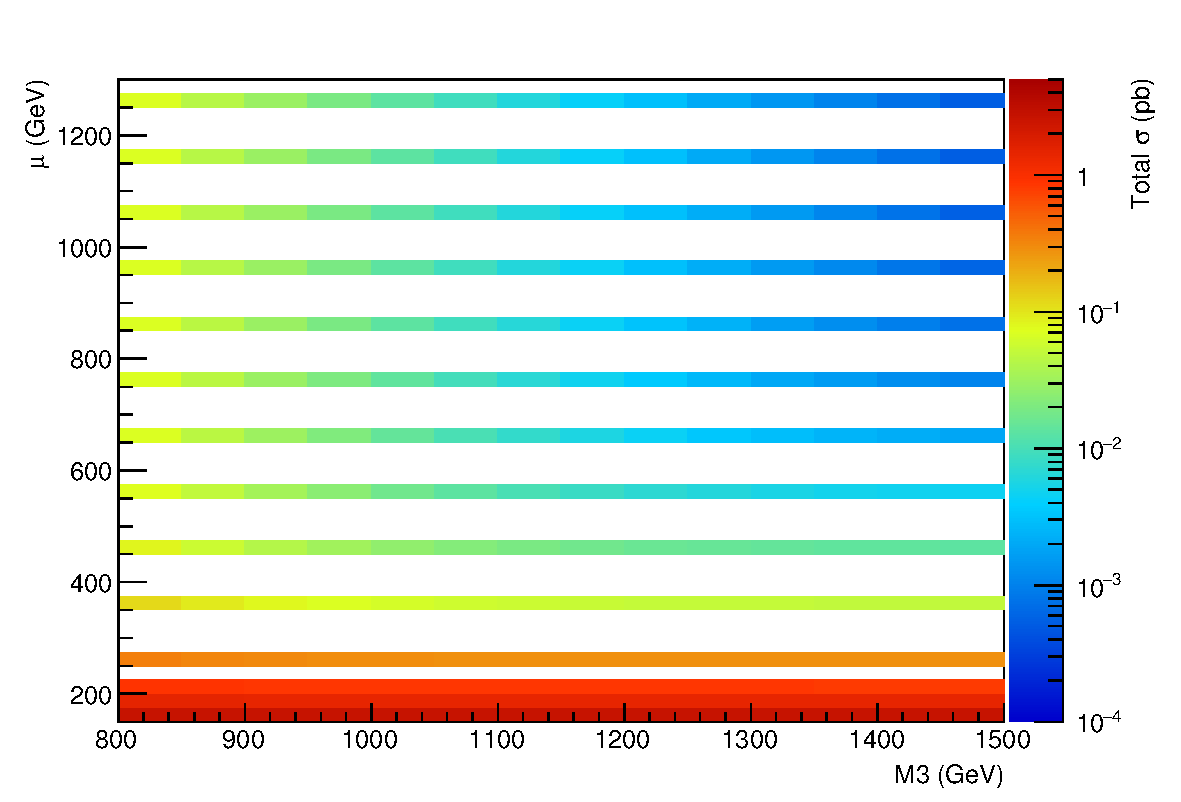
\includegraphics[width=0.49\textwidth]{figures/SigXsec_total}
%%   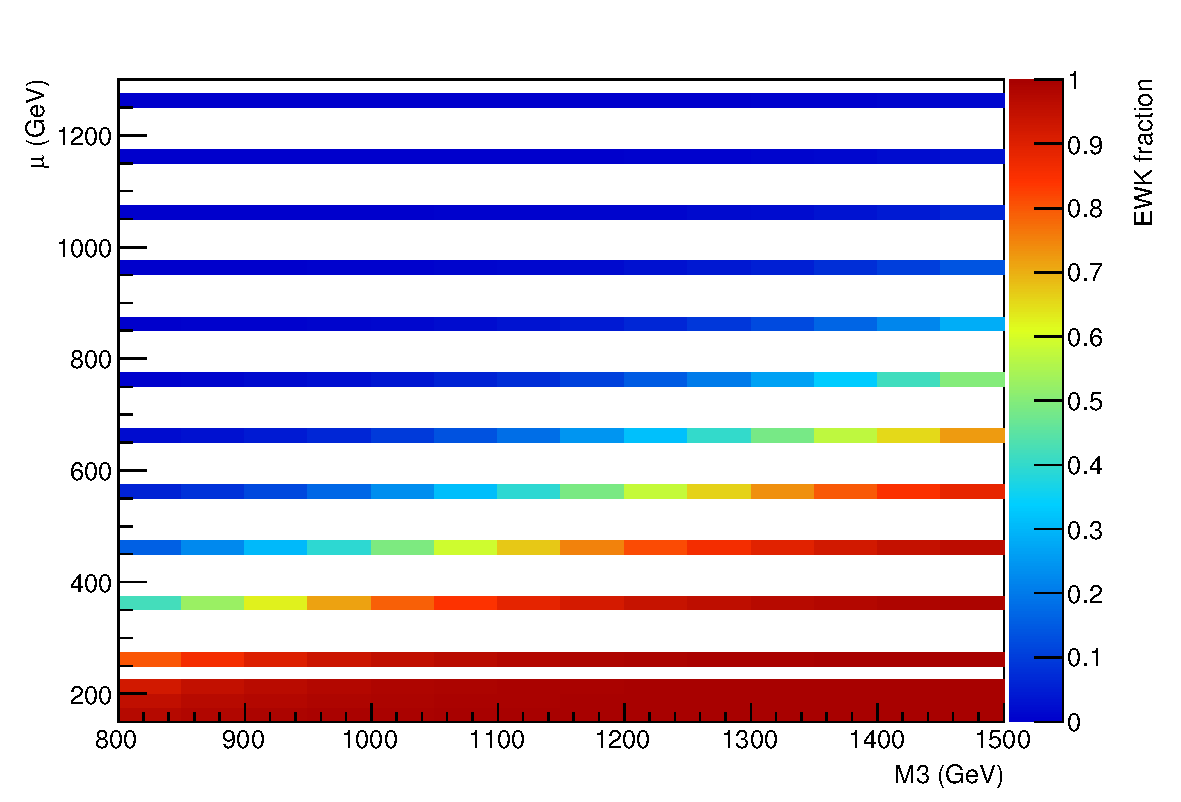
\includegraphics[width=0.49\textwidth]{figures/SigXsec_ewkFrac}
%%   \caption{Sección eficaz total (izquierda) y fracción relativa
%%     de producción EWK (derecha).}
%%   \label{fig:signal_xs_total}
%% \end{figure}

\section{Fondos del SM}
\label{sec:bkg_samples}

%% Existen muchos procesos del {\SM} que pueden aparentar
%% una señal de SUSY con fotones, jets y energía faltante.
%% Estos pueden dividirse en varias categorías:

%% \begin{itemize}
%% \item {\MET} real (EWK)
%%   \begin{itemize}
%%   \item $\gamma$ real
%%     \begin{itemize}
%%     \item $Z(\to\nu\nu)+\gamma$
%%     \item $W(\to\tau\nu)+\gamma$, hadronic $\tau$-decay
%%     \item $W(\to e\nu)+\gamma$, the e is not reconstructed
%%     \item $W(\to\mu\nu)+\gamma$ and $W(\to\tau\nu)+\gamma$, the $\mu / \tau$ is not reconstructed
%%     \item $t\bar{t}+\gamma$,  the e$/ \mu$ (when produced) is not reconstructed
%%     \end{itemize}

%%   \item Electron$/$Jet faking photon
%%     \begin{itemize}
%%     \item $W(\to l\nu)$+jets
%%     \item $Z(\to \nu\nu)+$jets
%%     \item $t\bar{t}$
%%     \item dibosons
%%     \end{itemize}
%%   \end{itemize}

%% \item {\MET} instrumental
%%   \begin{itemize}
%%   \item $\gamma$ real ($\gamma+$jets)
%%   \item $\gamma$ falso (multijet, $Z(\to ll)+$jets)
%%   \end{itemize}
%% \end{itemize}

%% Las muestras simuladas con MC utilizadas en este analisis se describen
%% a continuacion. Como se discutira en la {\Sec} \ref{sec:background_estimation},
%% la contaminacion de fotones mal dentificados provenientes de jets y electrones
%% es estimado con metodos basados en datos. Sin embargo, las muestras MC tambien
%% han sido consideradas en estos casos para los estudios de optimizacion y la
%% evaluacion de las incertezas sistematicas.

%% \subsection{W/Z$+\gamma$}

%% Se espera que la produccion de {\wgam} y {\zgam} sea un fondo importante
%% para esta busqueda. Ambas muestras fueron generadas usando el generador
%% de eventos {\sherpa} v1.4.1 \cite{SherpaGen}, con hasta 3 partones en el
%% ME+PS y usando las funciones de densidad partonica CT10.
%% La combinacion de los elementos de matriz con las lluvias partonicas
%% es realizada de acuerdo a un procedimiento mejorado CKKW \cite{Catani:2001cc,Krauss:2002up}.
%% Un filtro a nivel generados es aplicado requiriendo al menos un foton
%% con $\pt > 80(70) \gev$ en el estado final de las muestras de {\wgam} (\zgam).
%% %option1
%% %Only leptonic decays of the Z were considered, including its invisible decay Z$\to\nu\nu$. Additional samples of \wgamma events with some variation of the simulation settings were used to compute systematic uncertainties on the expected yields for this background. All \Vgamma samples are listed in {\tab} \ref{tab:bkg_wzgamma_samples}.
%% %option2
%% Todos los decaimientos leptonicos del boson $Z$ fueron considerados,
%% incluyendo el decaimiento invisible $Z\to\nu\nu$.
%% Tambien se tuvo en cuenta un muestra de $V(\to qq)+\gamma  (V=W,Z/\gamma*)$
%% debido a que cierta energia faltante real puede  ser producida en el caso
%% de heavy flavour decays.
%% %Their contribution had been found negligible in all regions here considered. \tosolve{CHECK!}
%% %

%% \begin{table}[ht!]
%%   \centering
%%   \caption{Muestras de W/Z$+\gamma$ utilizadas en este analisis.
%%     La seccion eficas a LO se especifica para cada modo de decaimiento,
%%     al igual que los factores $k$, y las eficiencias del filtro.
%%     La luminosidad integrada correspondiente a la estadistica total
%%     de cada muestra esta tambien presente.}
%%   %\includegraphics[width=1\textwidth]{figures/tabla}
%%   \begin{tabular}{ l | c | c | c | c }
%%     \hline
%%     \hline
%%     Proceso (ID) & $\sigma~[pb]$ & $k$ & Eficiencia & $L [fb^{-1}]$ \\
%%     \hline
%%     {\wenugam} {\sherpa} (126741) &  0.7193  &  1.0  &  1.0  &  695.16 \\
%%     {\wmunugam} {\sherpa}  (126744) &  0.7178  &  1.0  &  1.0  &  696.56 \\
%%     {\wtaunugam} {\sherpa}  (158727) &  0.7199  &  1.0  &  1.0  &  694.57 \\
%%     {\zeegam} {\sherpa}  (158728) &  0.1861  &  1.0  &  1.0  &  1069.53 \\
%%     {\zmumugam} {\sherpa}  (158729) &  0.1858  &  1.0  &  1.0  &  1076.71 \\
%%     {\ztautaugam} {\sherpa}  (158730) &  0.1858  &  1.0  &  1.0  &  1076.19 \\
%%     {\znunugam} {\sherpa}  (126022) &  0.7625  &  1.0  &  1.0  &  655.74 \\
%%   %%   % in case we use this in the end 'option2'
%%     {\vqqgam} {\sherpa}  (164438) &  6.756  &  1.0  &  1.0  &  89.0 \\
%%   %%   \hline
%%   %%   \hline
%%   %%   \multicolumn{5}{l}{Systematics variations} \\
%%   %%   \hline
%%   %%    \wenugam (fact. 0.25x) \sherpa (204733) &  0.7193  &  1.0  &  1.0  &  278.05 \\
%%   %%    \wenugam (fact. 4x) \sherpa (204734) &  0.7193  &  1.0  &  1.0  &  278.05 \\
%%   %%    \wenugam (renorm. 0.25x) \sherpa (204735) &  0.7193  &  1.0  &  1.0  &  278.05 \\
%%   %%    \wenugam (renorm. 4x) \sherpa (204736) &  0.7193  &  1.0  &  1.0  &  278.05 \\
%%   %%    \wenugam (ckkw 15) \sherpa (204731) &  0.7193  &  1.0  &  1.0  &  278.05 \\
%%   %%    \wenugam (ckkw 30) \sherpa (204732) &  0.7193  &  1.0  &  1.0  &  278.05 \\
%%   %%    \wmunugam (fact. 0.25x) \sherpa (204739) &  0.7193  &  1.0  &  1.0  &  278.63 \\
%%   %%    \wmunugam (fact. 4x) \sherpa (204740) &  0.7193  &  1.0  &  1.0  &  278.63 \\
%%   %%    \wmunugam (renorm. 0.25x) \sherpa (204741) &  0.7193  &  1.0  &  1.0  &  278.63 \\
%%   %%    \wmunugam (renorm. 4x) \sherpa (204742) &  0.7193  &  1.0  &  1.0  &  278.63 \\
%%   %%    \wmunugam (ckkw 15) \sherpa (204737) &  0.7193  &  1.0  &  1.0  &  278.63 \\
%%   %%    \wmunugam (ckkw 30) \sherpa (204738) &  0.7193  &  1.0  &  1.0  &  278.63 \\
%%   %%    \wtaunugam (fact. 0.25x) \sherpa (204745) &  0.7193  &  1.0  &  1.0  &  277.81 \\
%%   %%    \wtaunugam (fact. 4x) \sherpa (204746) &  0.7193  &  1.0  &  1.0  &  277.81 \\
%%   %%    \wtaunugam (renorm. 0.25x) \sherpa (204747) &  0.7193  &  1.0  &  1.0  &  277.81 \\
%%   %%    \wtaunugam (renorm. 4x) \sherpa (204748) &  0.7193  &  1.0  &  1.0  &  277.81 \\
%%   %%    \wtaunugam (ckkw 15) \sherpa (204743) &  0.7193  &  1.0  &  1.0  &  277.81 \\
%%   %%    \wtaunugam (ckkw 30) \sherpa (204744) &  0.7193  &  1.0  &  1.0  &  277.81 \\
%%     \hline
%%     \hline
%%   \end{tabular}
%%   \label{tab:bkg_wzgamma_samples}
%% \end{table}

%% \subsubsection{W/Z+jets} \label{mc_wzjets}

%% Se espera que la produccion de W$^{\pm}$ y bosones $Z$ en asociacion con jets
%% contribuya a esta busqueda, con los fotones provenientes de electrones y jets
%% mal identificados. Especialemente para los segundos, esta contaminacion no esta
%% bien descripta por el MC. Por esta razon se utilizan metodos basados en datos
%% para estimar su contirbucion en las diferentes regiones de senal y control, como
%% se describe en el Capítulo \ref{cap:fondos}. De igual maner varias muestras de MC
%% fueron consideradas para validar los metodos.

%% Como se describe en el Capítulo \ref{cap:seleccion} la seleccion de senal involucra
%% muchos jets en el estado final, es importante modelar los estados final multipartonicos
%% de forma adecuada. Con esto en mente, el generador de events {alpgen} (version 2.14)
%% fue utilizado, incluyendo los efectos EWK y QCD a LO para los procesos de interaccion
%% fuerte multipartonicos. La produccion de jets fue generada for up to five-parton
%% matrix elements. Este generados fue interfaceado con {\herwig} version 6.5.2
%% para la simulacion de las lluvias y los procesos de fragmentacion y con {\jimmy}
%% para la simulacion de los eventos subyacentes. Las funciones de densidad partonica
%% utilizadas fueron las CTEQ6L1. La normalizacion a la luminosidad integrada acumulada
%% fue hecha escalenado la seccion eficas mostrada en la {\tab} \ref{tab:bkg_wzjets_samples}
%% usando calculos QCD a NNLO de el programa FEWZ \cite{Anastasiou:2003ds}.
%% En cada caso los mismos factores de normalizacion fueron aplicados a los elementos
%% de matriz de {\alpgen}.
%% %%applied for all \alpgen matrix element parton multiplicities.
%% Finalmente, se realiza la remocion de eventos para evitar el conteo doble de eventos
%% que ya fueron tenidos en cuenta por las muestras de Z$\gamma$ y W$\gamma$.
%% Para esto, los eventos de $W(Z)+\text{jets}$ con fotones con $\pt > 80(70)\gev$
%% y $\Delta{\rm R}(e/\mu/\tau/$light-quarks$, \gamma) > 0.1$ fueron removidos
%% de las muestras.

%% \begin{table}[ht!]
%%   \centering
%%   \caption{Muestras de $W/Z+\text{jets}$ utilizadas en este analisis.
%%     La seccion eficas a LO para cada modo de decaimiento, los factores $k$
%%     (para la normalizacion NLO) y las eficiencias del filtro son reportadas,
%%     asi como tabine la luminosidad integrada correspondiente a la estadistica
%%     total de cada muestra.}
%%   \begin{tabular}{ l | c | c | c | c }
%%     \hline
%%     \hline
%%     Proceso (ID) & $\sigma~[pb]$ & k-factor & filter eff. & $\int{\mathcal{L}dt}~[fb^{-1}]$ \\
%%     \hline
%%     \zeenj{0}  \alpgen+\pythia (117650) & 718.89 & 1.18 & 1 & 7.80 \\
%% %    \zeenj{1}  \alpgen+\pythia (117651) & 175.60 & 1.18 & 1 & 6.42 \\
%% %    \zeenj{2}  \alpgen+\pythia (117652) & 58.846 & 1.18 & 1 & 5.83 \\
%% %    \zeenj{3}  \alpgen+\pythia (117653) & 15.56   & 1.18 & 1 & 5.99 \\
%% %    \zeenj{4}  \alpgen+\pythia (117654) & 3.9322 & 1.18 & 1 & 6.47 \\
%% %    \zeenj{5}  \alpgen+\pythia (117655) & 1.1994 & 1.18 & 1 & 7.07 \\
%% %    \zmmnj{0}  \alpgen+\pythia (117660) & 718.89 & 1.18 & 1 & 7.79 \\
%% %    \zmmnj{1}  \alpgen+\pythia (117661) & 175.81 & 1.18 & 1 & 6.43 \\
%% %    \zmmnj{2}  \alpgen+\pythia (117662) & 58.805 & 1.18 & 1 & 5.84 \\
%% %    \zmmnj{3}  \alpgen+\pythia (117663) & 15.589 & 1.18 & 1 & 5.98 \\
%% %    \zmmnj{4}  \alpgen+\pythia (117664) & 3.9072 & 1.18 & 1 & 6.51 \\
%% %    \zmmnj{5}  \alpgen+\pythia (117665) & 1.1933 & 1.18 & 1 & 7.10 \\
%% %    \zttnj{0} \alpgen+\pythia (117670) & 718.85 & 1.18 & 1 & 7.80 \\
%% %    \zttnj{1} \alpgen+\pythia (117671) & 175.83 & 1.18 & 1 & 6.43 \\
%% %    \zttnj{2} \alpgen+\pythia (117672) & 58.630 & 1.18 & 1 & 5.85 \\
%% %    \zttnj{3} \alpgen+\pythia (117673) & 15.508 & 1.18 & 1 & 5.96 \\
%% %    \zttnj{4} \alpgen+\pythia (117674) & 3.9526 & 1.18 & 1 & 6.43 \\
%% %    \zttnj{5} \alpgen+\pythia (117675) & 1.1805 & 1.18 & 1 & 7.18 \\
%%     \zeenj{0}  \alpgen+\jimmy (107650) & 711.77 & 1.23 & 1 & 7.548 \\
%%     \zeenj{1}  \alpgen+\jimmy (107651) & 155.17 & 1.23 & 1 & 6.994 \\
%%     \zeenj{2}  \alpgen+\jimmy (107652) & 48.745 & 1.23 & 1 & 6.746 \\
%%     \zeenj{3}  \alpgen+\jimmy (107653) & 14.225 & 1.23 & 1 & 6.286 \\
%%     \zeenj{4}  \alpgen+\jimmy (107654) & 3.7595 & 1.23 & 1 & 6.487 \\
%%     \zeenj{5}  \alpgen+\jimmy (107655) & 1.0945 & 1.23 & 1 & 7.428 \\
%%     \zmmnj{0}  \alpgen+\jimmy (107660) & 712.11 & 1.23 & 1 & 7.557 \\
%%     \zmmnj{1}  \alpgen+\jimmy (107661) & 154.77 & 1.23 & 1 & 7.011 \\
%%     \zmmnj{2}  \alpgen+\jimmy (107662) & 48.912 & 1.23 & 1 & 6.731 \\
%%     \zmmnj{3}  \alpgen+\jimmy (107663) & 14.226 & 1.23 & 1 & 6.286 \\
%%     \zmmnj{4}  \alpgen+\jimmy (107664) & 3.7838 & 1.23 & 1 & 6.445 \\
%%     \zmmnj{5}  \alpgen+\jimmy (107665) & 1.1148 & 1.23 & 1 & 7.292 \\
%%     \zttnj{0} \alpgen+\jimmy (107670) & 711.81 & 1.23 & 1 &  7.560 \\
%%     \zttnj{1} \alpgen+\jimmy (107671) & 155.13 & 1.23 & 1 &  6.996 \\
%%     \zttnj{2} \alpgen+\jimmy (107672) & 48.804 & 1.23 & 1 &  6.746 \\
%%     \zttnj{3} \alpgen+\jimmy (107673) & 14.160 & 1.23 & 1 &  6.315 \\
%%     \zttnj{4} \alpgen+\jimmy (107674) & 3.7744 & 1.23 & 1 &  6.462 \\
%%     \zttnj{5} \alpgen+\jimmy (107675) & 1.1163 & 1.23 & 1 &  7.283 \\
%%     \hline
%%     \hline
%%     \wenunj{0}  \alpgen+\jimmy (107680) &8037.10   & 1.186 & 1 & 0.362 \\
%%     \wenunj{1}  \alpgen+\jimmy (107681) &1579.20   & 1.186 & 1 & 1.334 \\
%%     \wenunj{2}  \alpgen+\jimmy (107682) &477.20     & 1.186 & 1 & 6.661 \\
%%     \wenunj{3}  \alpgen+\jimmy (107683) &133.93     & 1.186 & 1 & 6.358 \\
%%     \wenunj{4}  \alpgen+\jimmy (107684) &35.62       & 1.186 & 1 &  5.917\\
%%     \wenunj{5}  \alpgen+\jimmy (107685) &10.55       & 1.186 & 1 &  5.592\\
%%     \wmnunj{0}  \alpgen+\jimmy (107690) &8040.00 & 1.186 & 1 &  0.363\\
%%     \wmnunj{1}  \alpgen+\jimmy (107691) &1580.30 & 1.186 & 1 &  1.333\\
%%     \wmnunj{2}  \alpgen+\jimmy (107692) &477.50   & 1.186 & 1 &  6.656\\
%%     \wmnunj{3}  \alpgen+\jimmy (107693) &133.94   & 1.186 & 1 &  6.357\\
%%     \wmnunj{4}  \alpgen+\jimmy (107694) &35.64      & 1.186 & 1 &  6.033\\
%%     \wmnunj{5}  \alpgen+\jimmy (107695) &10.57      & 1.186 & 1 &  1.595\\
%%     \wtnunj{0} \alpgen+\jimmy (107700)    &8035.80  & 1.186 & 1 & 0.353 \\
%%     \wtnunj{1} \alpgen+\jimmy (107701)    &1579.80  & 1.186 & 1 & 1.307 \\
%%     \wtnunj{2} \alpgen+\jimmy (107702)    &477.55    & 1.186 & 1 &  6.567\\
%%     \wtnunj{3} \alpgen+\jimmy (107703)    &133.79    & 1.186 & 1 &  6.365\\
%%     \wtnunj{4} \alpgen+\jimmy (107704)    &35.58      & 1.186 & 1 &  5.921\\
%%     \wtnunj{5} \alpgen+\jimmy (107705)    &10.54      & 1.186 & 1 &  5.199\\
%%     \hline
%%     \hline
%%   \end{tabular}
%%   \label{tab:bkg_wzjets_samples}
%% \end{table}


%% \subsubsection{Top pair ($+\gam$) production}\label{sec:mcttbargam}

%% Another important background to this analysis is \ttgam. This MC sample was generated using the
%% {\madgraph} \cite{Alwall:2007st} MC generator and the CTEQ6L1 PDF. %No fully hadronic \ttbar\ was included.
%%   {\pythiasix} \cite{pythia} was used for parton showering, fragmentation and underlying event
%% simulation. Additional photon radiation was added with
%% {\photos} \cite{photos}, and tau leptons were decayed with
%% {\tauola} \cite{tauola}. The truth-level photons were required to have
%% $\pt > 80 \gev$. To avoid kinematic effects introduced by the filter, the photon \pt\ cut on the reconstructed sample was raised to 95 \gev.
%% A $k$-factor of $1.9 \pm 0.4$ is used \cite{Melnikov:2011ta, tth}. %This was calculated by
%% %the theorists with the particular generator-level cuts used to                                                                                                                     %generate this MC sample.

%% Simulation details are given in {\tab} \ref{tab:bkg_ttbar_samples}. The MC samples with IDs 202332--202337 are truth-only systematic variation samples, used to estimate systematic
%% uncertainties as explained in {\Sec} \ref{sec:syst_ttbargamma}.


%% % NOT ANYMORE , but explained later why
%% %As described in {\sec} \ref{}, the normalization of this sample was extracted together with that for %W$+\gamma$ events by fitting
%% %simultaneously the two MC to data in specifically designed control regions.

%% %More information can be found in
%% %Ref.~\cite{ttbargammaSupport}.

%% La produccion de {\ttbar}, donde los electrones o los jets
%% son mal identificados como fotones es una fuente de fondo que
%% vale la pena considerar.

%% %% Although both fakes contamination were estimated from the data, simulated events were used at the  optimization stage
%% %% and for cross checks of the data-driven methods. The MC sample was generated using the
%% %% {\powheg} \cite{Nason:2004rx,Frixione:2007vw,Alioli:2010xd} generator, with the parton showering and fragmentation done in \pythia.
%% %% The new Perugia 2011C tune \footnote{see some details at \url{https://twiki.cern.ch/twiki/bin/viewauth/AtlasProtected/P2011C}.} was used for the underlying event,
%% %%  with the CTEQ6L1 LO* set of PDFs. Additional photon radiation was added with {\photos} \cite{photos}.
%% %% Overlap removal is performed to prevent double-counting the phase-space
%% %% covered by the {\ttgam} MC sample. Events with truth prompt photons with
%% %% $\pt > 95 \gev$ and $\Delta{\rm R}(e/\mu/\tau/g/$light-quarks$, \gamma) > 0.1$ are removed from the \ttbar\ sample.


%% %% ttbar normalization??

%% %The nominal normalization of this sample is based on a cross section
%% %calculated at approximate NNLO in QCD using Hathor
%% %1.2~\cite{Aliev:2010zk} using the MSTW2008 \unit[90]{\%} NNLO PDF
%% %sets~\cite{MSTW2008} and incorporating PDF+$\alpha_S$ uncertainties
%% %according to the MSTW prescription~\cite{Martin:2009bu}. The value is
%% %cross checked with the NLO+NNLL calculation of Cacciari et
%% %al.~\cite{Cacciari:2011hy} as implemented in Top++
%% %1.0~\cite{Czakon:2011xx}. An uncertainty of \unit[11.0]{\%} is assigned
%% %to the NNLO cross section (which incorporates the mass uncertainty).
%% %


%% \begin{table}[ht!]
%%   \centering
%%   \caption{\ttgam\ samples used for the analysis. The LO cross-section for specified decay mode, k-factors (for NLO normalisation) and filter efficiencies are reported. The integrated luminosities corresponding to the total statistics in each sample are also given. The bottom group of samples was used to study systematic uncertainties.}
%%   \includegraphics[width=1\textwidth]{figures/tabla}
%%   %% \begin{tabular}{ l | c | c | c | c }
%%   %%   \hline
%%   %%   \hline
%%   %%   Process (ID) & $\sigma~[pb]$ & k-factor & filter eff. & $\int{\mathcal{L}dt}~[fb^{-1}]$ \\
%%   %%   \hline
%%   %%   \hline
%%   %%   \ttbar\ \powheg+\pythia (117050)  & 253.00 & 1 & 0.543 & 580 \\
%%   %%   \hline
%%   %%   %    \ttbargam noAllHad \madgraph (164439) & 0.092363 & 1.9 & 1 & 1139.7 \\
%%   %%   \ttbargam\ noAllHad \madgraph (177998) & 0.09873 & 1.9 & 1 & 1066.2 \\
%%   %%   \ttbargam\ AllHad \madgraph (174382) & 0.068599 & 1.9 & 1 & 1534.5 \\
%%   %%   \hline
%%   %%   \hline
%%   %%   \multicolumn{5}{l}{Systematics variations} \\
%%   %%   \hline
%%   %%   \ttbargam\ noAllHad (scaleUP) \madgraph (202332) & 0.09873 & 1.9 & 1 & 1066.2 \\
%%   %%   \ttbargam\ noAllHad (scaleDN) \madgraph (202333) & 0.09873 & 1.9 & 1 & 1066.2 \\
%%   %%   \ttbargam\ noAllHad (alpsUP) \madgraph (202334) & 0.09873 & 1.9 & 1 & 1066.2 \\
%%   %%   \ttbargam\ noAllHad (alpsDN) \madgraph (202335) & 0.09873 & 1.9 & 1 & 1066.2 \\
%%   %%   \ttbargam\ noAllHad (moreFSR) \madgraph (202336) & 0.09873 & 1.9 & 1 & 1066.2 \\
%%   %%   \ttbargam\ noAllHad (lessFSR) \madgraph (202337) & 0.09873 & 1.9 & 1 & 1066.2 \\
%%   %%   \hline
%%   %%   \hline
%%   %% \end{tabular}
%%   \label{tab:bkg_ttbar_samples}
%% \end{table}

\subsubsection{Single top (+ $\gamma$)}

Single top con un foton asociado fue generado utilizando
Whizard 2.1.1 \cite{whizard, whizard2}, con 4-flavor/5-flavor
matching provided using Hoppet~\cite{hoppet}.\footnote{Thanks to
  abian Bach for providing an early version of the matching, which
  will be standard in Whizard 2.2.0.}
El foton extra photon could be in
%% either the single top production or the subsequent decays. Production
%% and decay, however, was treated separately, so interference effects
%% are ignored. {\pythia} \cite{pythia} was used for parton showering and
%% fragmentation. Additional photon radiation was added with
%% {\photos} \cite{photos}, and tau leptons were decayed with
%% {\tauola} \cite{tauola}.

%% %We used sample IDs 202621 and 202622 for \tchangamma production, and
%% %sample IDs 202623--202631 for \tWgamma production.

%% \begin{table}[ht!]
%%   \centering
%%   \caption{Single top and \tgam\ samples used for the analysis. The NNLO cross-section, filter efficiencies and the integrated luminosities corresponding to the total statistics in each sample are also given.}
%%   \includegraphics[width=1\textwidth]{figures/tabla}
%%   %% \begin{tabular}{ l | c | c | c }
%%   %%   \hline
%%   %%   \hline
%%   %%   Process (ID) & $\sigma~[pb]$ & filter eff. & $\int{\mathcal{L}dt}~[fb^{-1}]$ \\
%%   %%   \hline
%%   %%   t-channel \acermc (110101)  & 28.4 & 1 & 271 \\
%%   %%   Wt        \powheg (110140)  & 22.4 & 1 & 892 \\
%%   %%   s-channel \powheg (110119)  & 1.82 & 1 & 3299 \\
%%   %%   \hline
%%   %%   \hline
%%   %%   \tgam (t-channel) \wizhard+\pythia (202621)  & 0.187298 & 0.121980 & 4810 \\
%%   %%   \tgam (t-channel) \wizhard+\pythia (202622)  & 0.313866 & 0.012927 & 4930 \\
%%   %%   \hline
%%   %%   \twgam (dilep.) \wizhard+\pythia (202623)  & 0.012915  & 0.164370 & 4710 \\
%%   %%   \twgam (dilep. tDec) \wizhard+\pythia (202624)  & 0.014538  & 0.028748 & 12000 \\
%%   %%   \twgam (dilep. WDec) \wizhard+\pythia (202625)  & 0.010405  & 0.075489 & 6370 \\
%%   %%   \twgam (tlepWhad) \wizhard+\pythia (202626)  & 0.025825 & 0.162440 & 4770 \\
%%   %%   \twgam (tlepWhad tDec) \wizhard+\pythia (202627)  & 0.029084  & 0.027609 & 6230 \\
%%   %%   \twgam (tlepWhad WDec) \wizhard+\pythia (202628)  & 0.011594  & 0.064709 & 6660 \\
%%   %%   \twgam (thadWlep) \wizhard+\pythia (202629)  & 0.025817 & 0.161780 & 4790 \\
%%   %%   \twgam (thadWlep tDec) \wizhard+\pythia (202630)  & 0.020127  & 0.041977 & 5920 \\
%%   %%   \twgam (thadWlep WDec) \wizhard+\pythia (202631)  & 0.020788  & 0.075740 & 3180 \\
%%   %%   \hline
%%   %%   \hline
%%   %% \end{tabular}
%%   \label{tab:bkg_st_samples}
%% \end{table}

%% The single top process is a small background for this analysis, mostly
%% important for the control and validation regions. $Wt$ production (ID 110140) was generated using the \powheg, including full next-to-leading order QCD
%% corrections. Parton showering and fragmentation were simulated by
%% \pythia with the P2011C tune. The CT10 next-to-leading-order parton
%% set is used for the matrix element, the parton shower and the
%% underlying event. The samples were scaled to the cross section
%% calculated in \cite{Kidonakis:2010ux}. For $t$-channel
%% production, the MC samples with sample ID 110101 were used, with the
%% $W$ boson decaying leptonically. These were generated with
%% \acermc \cite{acer}, with parton showering and fragmentation performed
%% by {\pythia} with the P2011C tune and CTEQ6L1 PDF set.  The samples were
%% scaled to the cross section calculated by \cite{Kidonakis:2011wy}.
%% Single top produced by $s$-channel was not used because it was found
%% to be negligible.

%% Overlap between the single top and single top $\gamma$ samples has been removed.

\subsubsection{Direct $\gamma+$jets and QCD multijet}

%% %The QCD background is one of the main source of background in this analysis, particularly prompt photon events. The QCD contamination is in all cases a result of pathological events (jet faking a photon, badly reconstructed jet or photon making high \MET) for which the simulation is not reliable.
%% %For this reason this background is computed with a data driven approach, as explained in {\sec} \ref{sec:jetsmearing}. Several MC simulations are used anyways for consistency checks and to assess systematic uncertainties.

%% The QCD contamination is in all cases a result of pathological events
%% (jet faking a photon, badly reconstructed jet or photon making high \MET).
%% However, it is not expected to be a dominant source of background in the
%% phase space explored in this analysis. The contribution from events with
%% jets faking a photon is estimated with the data driven described in
%% {\Sec} \ref{sec:jetfakes}. The QCD multijet samples listed in {\tab}
%% \ref{tab:bkg_qcd_samples} were used for optimisation and preliminar
%% sensitivity studies. Prompt photon production was simulated with
%% with {\sherpa} v1.4.1 \cite{SherpaGen}, with up to four partons in the ME+PS
%% and using the CT10 set of parton density functions. The inclusive spectrum
%% is sliced in ranges of photon \pt\ to optimise the event generation.
%% Alternative samples were used to asses systematics uncertainties and
%% cross checks, generated with {\pythiaeight} (using CTEQ6L1) and {\alpgen}
%% v2.14 (with same config as V$+$jets events described in {\Sec} \ref{mc_wzjets}).
%% Further details are given in {\tab} \ref{tab:bkg_qcd_samples}.

%% \begin{table}[ht!]
%%   \centering
%%   \caption{Muestras de QCD {\gjet} y multijet utilizadas en este analisis.
%%     La seccion eficas a LO para cada modo de decaimiento,
%%     y las eficiencias del filtro son reportadas,
%%     asi como tabine la luminosidad integrada correspondiente a la estadistica
%%     total de cada muestra.}

%%   %% \includegraphics[width=1\textwidth]{figures/tabla}

%%    \begin{tabular}{ l | c | c | c }
%%     \hline
%%     \hline
%%     Proceso & $\sigma~[pb]$ & filter eff. & $\int{\mathcal{L}dt}~[fb^{-1}]$ \\
%%     \hline
%%     {\gjet} ($\pt>70\gev$)  &  2153.0  &  1.0  &  1.160 \\
%%     {\gjet} ($\pt>140\gev$) &  137.85  &  1.0  &  10.881 \\
%%     {\gjet} ($\pt>280\gev$) &  5.963  &  1.0  &  167.657 \\
%%     {\gjet} ($\pt>500\gev$) &  0.276  &  1.0  &  3617.291 \\
%%     {\gjet} ($\pt>800\gev$) &  0.0133  &  1.0  &  7492.807 \\
%%     {\gjet} ($\pt>1000\gev$) &  0.00238  &  1.0  &  41980.269 \\
%%     \hline

%%     \hline
%%     {\gjet} ($\pt>70\gev$)   &  3425000  &  $5.7 \times 10^{-4}$  &  1535.4  \\
%%     {\gjet} ($\pt>140\gev$)  &  122170  &  $9.7 \times 10^{-4}$  &  8449.2 \\
%%     {\gjet} ($\pt>280\gev$)  &  3348.7  &  $1.45 \times 10^{-3}$  &  206559.7 \\
%%     {\gjet} ($\pt>500\gev$)  &  115.63  &  $1.8 \times 10^{-3}$  &  4789097.0\\
%%     \hline

%%     \gjetnj{1} ($\pt>70\gev$) \alpgen+\jimmy  ( 156843 ) &  577.480  &  1.0  &  0.147 \\
%%     \gjetnj{1} ($\pt>140\gev$) \alpgen+\jimmy  ( 156839 ) &  26.198  &  1.0  &  3.626 \\
%%     \gjetnj{1} ($\pt>280\gev$) \alpgen+\jimmy  ( 156840 ) &  0.83119  &  1.0  &  30.077 \\
%%     \gjetnj{1} ($\pt>500\gev$) \alpgen+\jimmy  ( 156842 ) &  0.029141  &  1.0  &  343.159 \\

%%     % \gjetnj{2} ($\ptgam>35\gev$) \alpgen+\jimmy  ( 156846 ) &  4515.0  &  1.0  &  0.00886 \\
%%     \gjetnj{2} ($\pt>70\gev$) \alpgen+\jimmy  ( 156848 ) &  571.870  &  1.0  &  0.175 \\
%%     \gjetnj{2} ($\pt>140\gev$) \alpgen+\jimmy  ( 156844 ) &  38.671001  &  1.0  &  3.879 \\
%%     \gjetnj{2} ($\pt>280\gev$) \alpgen+\jimmy  ( 156845 ) &  1.6811  &  1.0  &  29.741 \\
%%     \gjetnj{2} ($\pt>500\gev$) \alpgen+\jimmy  ( 156847 ) &  0.075517  &  1.0  &  264.841 \\

%%     % \gjetnj{3} ($\ptgam>35\gev$) \alpgen+\jimmy  ( 156851 ) &  1717.0  &  1.0  &  0.00874 \\
%%     \gjetnj{3} ($\pt>70\gev$) \alpgen+\jimmy  ( 156853 ) &  306.10  &  1.0  &  0.049\\
%%     \gjetnj{3} ($\pt>140\gev$) \alpgen+\jimmy  ( 156849 ) &  28.57  &  1.0  &  5.250 \\
%%     \gjetnj{3} ($\pt>280\gev$) \alpgen+\jimmy  ( 156850 ) &  1.538  &  1.0  &  32.503 \\
%%     \gjetnj{3} ($\pt>500\gev$) \alpgen+\jimmy  ( 156852 ) &  0.077073  &  1.0  &  77.822 \\

%%     % \gjetnj{4} ($\ptgam>35\gev$) \alpgen+\jimmy  ( 156856 ) &  513.940002  &  1.0  &  0.00778 \\
%%     \gjetnj{4} ($\pt>70\gev$) \alpgen+\jimmy  ( 156858 ) &  115.850  &  1.0  &  0.216 \\
%%     \gjetnj{4} ($\pt>140\gev$) \alpgen+\jimmy  ( 156854 ) &  14.216  &  1.0  &  11.951 \\
%%     \gjetnj{4} ($\pt>280\gev$) \alpgen+\jimmy  ( 156855 ) &  0.9185  &  1.0  &  48.992 \\
%%     \gjetnj{4} ($\pt>500\gev$) \alpgen+\jimmy  ( 156857 ) &  0.0512  &  1.0  &  156.354 \\

%%     % \gjetnj{5} ($\ptgam>35\gev$) \alpgen+\jimmy  ( 156861 ) &  163.800003  &  1.0  &  0.0458 \\
%%     \gjetnj{5} ($\pt>70\gev$) \alpgen+\jimmy  ( 156859 ) &  7.00  &  1.0  &  18.569 \\
%%     \gjetnj{5} ($\pt>140\gev$) \alpgen+\jimmy  ( 156860 ) &  0.542  &  1.0  &  92.304 \\
%%     \gjetnj{5} ($\pt>280\gev$) \alpgen+\jimmy  ( 156862 ) &  0.0333  &  1.0  &  450.911 \\
%%     \gjetnj{5} ($\pt>500\gev$) \alpgen+\jimmy  ( 156863 ) &  44.334  &  1.0  &  0.970 \\
%%     \hline
%%     \hline
%%     JZ1W ($20 \gev < p^{\rm leading jet}_{\rm T} < 80 \gev$) \pythia (147911) &  $7.285 \times 10^{10}$ &  0.000129 & 0.00016 \\
%%     JZ2W ($80 \gev < p^{\rm leading jet}_{\rm T} < 200 \gev$) \pythia (147912) &  $2.634 \times 10^{7}$ &  0.003894 & 0.0142 \\
%%     JZ3W ($200 \gev < p^{\rm leading jet}_{\rm T} < 500 \gev$) \pythia (147913) &  $5.442 \times 10^{5}$ &  0.001219 & 2.26 \\
%%     JZ4W ($500 \gev < p^{\rm leading jet}_{\rm T} < 1000 \gev$) \pythia (147914) &  $6.445 \times 10^{3}$ &  0.000708 & 328 \\
%%     JZ5W ($1000 \gev < p^{\rm leading jet}_{\rm T} < 1500 \gev$) \pythia (147915) &  39.74 &  0.002152 & 17400 \\
%%     JZ6W ($1500 \gev < p^{\rm leading jet}_{\rm T} < 2000 \gev$) \pythia (147916) &  0.4161 &  0.004684 & $7.68 \times 10^{5}$ \\
%%     JZ7W ($p^{\rm leading jet}_{\rm T} > 2000 \gev$) \pythia (147917) &  0.04064 &  0.0146 & $2.52\times 10^{6}$ \\
%%     \hline
%%   \end{tabular}
%%   \label{tab:bkg_qcd_samples}
%% \end{table}

\subsubsection{Dibosons}

Los procesos de diboson (WW, WZ, y ZZ) fueron generados utilizando
{\sherpa} y usando la PDF CT10, con la seccion eficaz provista por
MCFM \cite{Campbell:2011bn}. Solo los decaimientos leptonicos para
ambos bosones fueron considerados.

\begin{table}[ht!]
  \centering
  \caption{Muestras de Diboson utilizadas en este analisis.
    La seccion eficas a LO para cada modo de decaimiento, los factores $k$
    (para la normalizacion NLO) y las eficiencias del filtro son reportadas,
    asi como tabine la luminosidad integrada correspondiente a la estadistica
    total de cada muestra.}

  \begin{tabular}{ l | c | c | c | c }
    \hline
    \hline
    Proceso & $\sigma [pb]$ & factor $k$ & Eficiencia & $L [fb^{-1}]$ \\
    \hline
    %% $WW(2l2\nu)$ \sherpa (126892)  & 5.50 & 1.07 & 1 & 458.9 \\
    %% $WZ(3l)$ \sherpa (126893) & 9.75 & 1.06 & 1 & 261.1 \\
    %% $ZZ(4l)$ \sherpa (126894)  & 8.74 & 1.11 & 1  &  185.6 \\
    %% $ZZ(2l2\nu)$ \sherpa (126895)  & 0.50 & 1.14 & 1 &  1590.8 \\
    $WW(ll\nu\nu)$       & 5.2963  & 1.06 & 1 & 1400 \\
    $ZZ(ll\nu\nu)$       & 0.49434 & 1.05 & 1 & 1700 \\
    $WZ(lll\nu)$         & 9.74456 & 1.05 & 1 & 260 \\
    $WZ(l\nu\nu\nu)$     & 1.4047  & 1.05 & 1 & 270 \\
    $ZW(eeqq)$           & 1.4648  & 1.05 & 1 & 110 \\
    $ZZ(eeqq)$           & 0.24672 & 1    & 1 & 120 \\
    $ZW(\mu\mu qq)$      & 1.4634  & 1.05 & 1 & 110 \\
    $ZZ(\mu\mu qq)$      & 0.24757 & 1    & 1 & 120 \\
    $ZW(\tau\tau qq)$    & 1.4523  & 1.05 & 1 & 120 \\
    $ZZ(\tau\tau qq)$    & 0.24167 & 1    & 1 & 120 \\
    $ZW(\nu\nu qq)$      & 2.6972  & 1.05 & 1 & 64 \\
    $ZZ(\nu\nu qq)$      & 1.7440  & 1    & 1 & 69 \\
    $WW(e\nu qq)$        & 7.2854  & 1.06 & 1 & 100 \\
    $WZ(e\nu qq)$        & 1.9036  & 1.05 & 1 & 110 \\
    $WW(\mu\nu qq)$      & 7.2974  & 1.06 & 1 & 100 \\
    $WZ(\mu\nu qq)$      & 1.9057  & 1.05 & 1 & 100 \\
    $WW(\tau\nu qq)$     & 7.2741  & 1.06 & 1 & 100 \\
    $WZ(\tau\nu qq)$     & 1.9152  & 1.05 & 1 & 100 \\
    \hline
    \hline
  \end{tabular}
  \label{tab:bkg_diboson_samples}
 \end{table}
